\begin{table}[htbp]
    \centering
    \caption{Deployment Schemes}
    \label{tab:deployment_schemes}
    \begin{tabular}{p{0.3\linewidth} p{0.6\linewidth}}
        \hline
        \textbf{Scheme} & \textbf{Description} \\
        \hline
        Greedy Deployment & Deploy the largest reactor first at each time step, fill in the remaining capacity with the next smallest, and so on. \\
        \vspace{0.4mm}
        Capped Deployment & There is a single-number capacity for one or more of the reactor models. \\
        \vspace{0.4mm}
        Pre-Determined Distribution Deployment & One or more reactors have a preset distribution, and a smaller capacity model fills in the gaps. \\
        \vspace{0.4mm}
        Random Deployment & Uses a date and hour as seed to randomly sample the reactors list. \\
        \vspace{0.4mm}
        Initially Random, Greedy Deployment & Randomly deploys reactors until a reactor bigger than the remaining capacity is proposed for each year, then fills remaining capacity with a greedy algorithm. \\
        \hline
    \end{tabular}
\end{table}

We apply each of these deployment schemes to a series of demand growth scenarios based on two predictions. The \gls{eia} publishes demand expansion projections for the totality of \gls{usa} .
% source name and citation with

\begin{table}[htbp]
    \centering
    \caption{Demand Growth Scenarios}
    \label{tab:demand_scenarios}
    \begin{tabular}{c c c}
        \hline
        \textbf{Demand Growth} & \textbf{Range} & \textbf{Source}\\
        \hline
        No growth & 0\% & na\\
        Low growth & 1\%, 5\%, 10\%, 15\% & (eia)\\
        High growth & 100\%, 200\% & (liftoff)\\
        \hline
    \end{tabular}
\end{table}

\section{Greedy Deployment}
% describe the algorithm in detail
In this deployment scheme, the largest reactor is deployed first until another
deployment of that reactor would exceed the demand. Then the next largest
reactor is deployed in the same pattern until the next deployment of the
smallest reactor would exceed the demand. This scheme is not a proxy for
strategic decisions by individual actors, it merely meets the demand in a
roughly efficient manner.

\begin{figure}[!htbp]
    \centering
    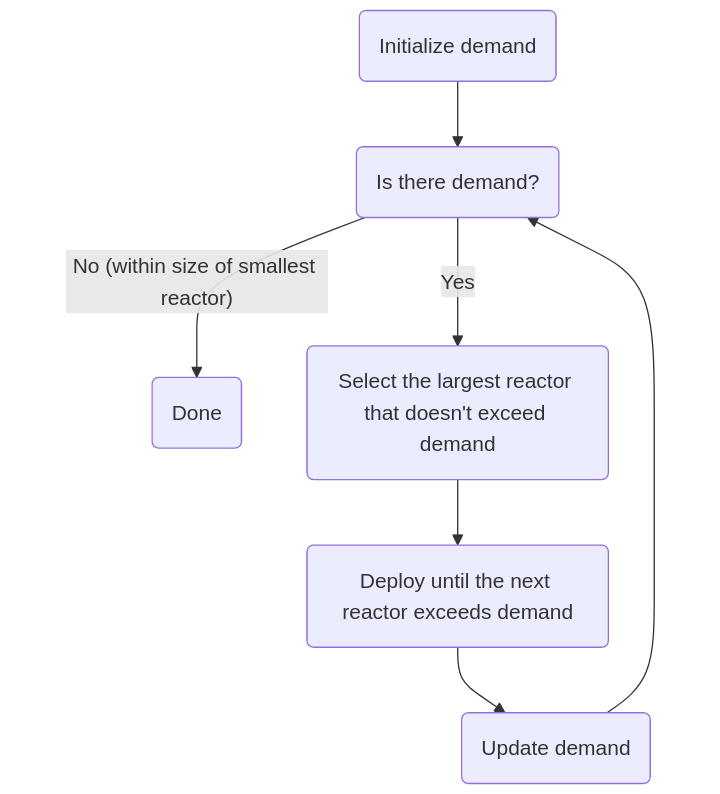
\includegraphics[scale=0.4]{images/schemes/greedy_diagram.png}
    \caption{Greedy Deployment Diagram}
    \label{fig:greedy_diagram}
\end{figure}

% what are the realistic and the unrealistic parts

% when does it over or under perform

\section{Capped Deployment}
% describe the algorithm in detail
To use this deployment scheme, a user needs to have some idea of the supply chain constraints that will limit the deployment of the reactors they are deploying.

\begin{figure}[!htbp]
    \centering
    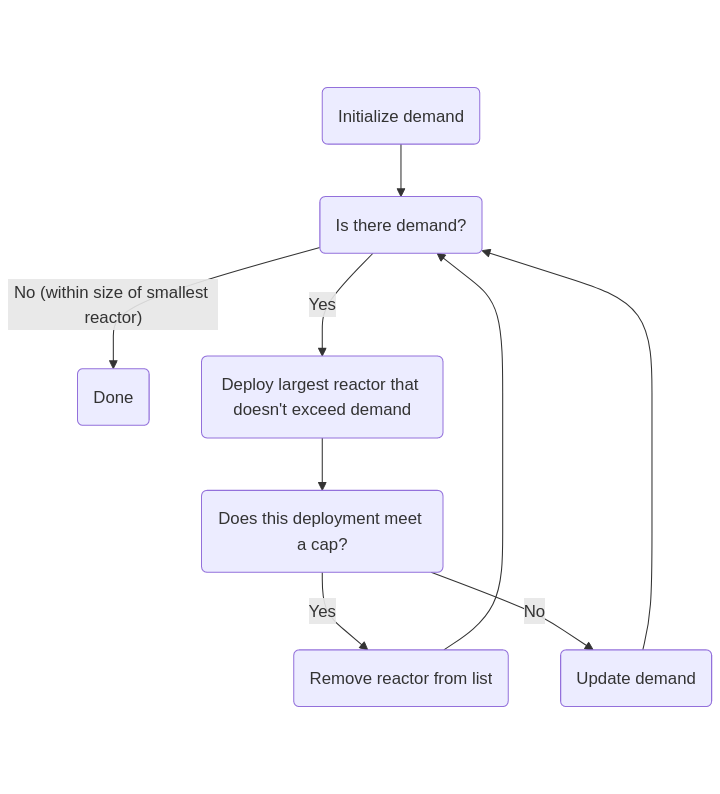
\includegraphics[scale=0.4]{images/schemes/cap_diagram.png}
    \caption{Capped Deployment Diagram}
    \label{fig:cap_diagram}
\end{figure}

% what are the realistic and the unrealistic parts
The realism of this deployment scheme mirrors some elements of the pre-determined distribution (this is a flat distribution after all), but the cap is a less granular way to account for supply chain constraints

% when does it over or under perform

\section{Pre-Determined Distribution Deployment}
% describe the algorithm in detail
This deployment scheme allows users to incorporate the projections and
commitments of rate payers and utilities by setting a distribution over the
time of the simulation. In this scheme the distribution serves as a cap to the
number of reactors deployed in a time step, and reactors are preferentially
deployed first to meet those caps. After that has been completed, the remaining
reactors without caps are deployed to meet the demand. In this way, we are able
to incorporate knowledge of supply chain constraints for specific technologies
without having to model the supply chain in detail.
% would be great to find some sources for this, and see what the literature says

\begin{figure}[!htbp]
    \centering
    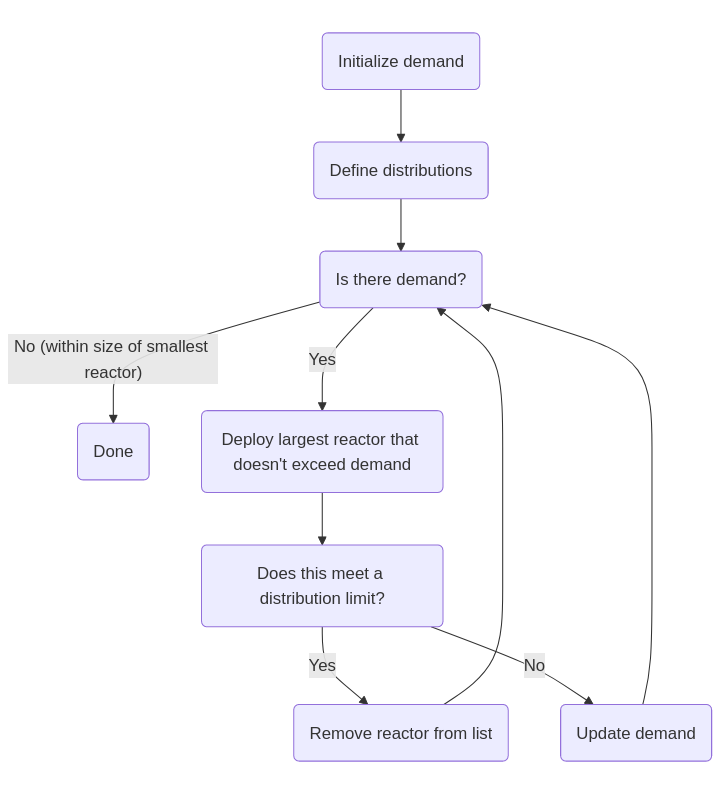
\includegraphics[scale=0.4]{images/schemes/pre_det_diagram.png}
    \caption{Pre-Determined Distribution Deployment Diagram}
    \label{fig:pre_det_diagram}
\end{figure}

% what are the realistic and the unrealistic parts

% when does it over or under perform
This scheme is most useful when there are known commitments to specific technologies.

\section{Random Deployment}
% describe the algorithm in detail

% what are the realistic and the unrealistic parts
Advanced reactor concepts, like the ones outlined in this work, are often designed for a different use-cases. ((((((((((((cite))))))))))))


The deployment of these reactors is a complex problem that requires a nuanced
understanding of the energy market, the regulatory environment, the intended
use of the technology, and the technical capabilities of the reactor. This
random deployment is a proxy for the complexity of the real-world deployment
problem, but does not include the nuance of future user needs, which will drive
the strategic decisions that utilities and rate payers behind the meter make in
their reactor choices.

This deployment scheme has the potential to capture some of the complexities in
overall market development, but the extent that these details are captured is
not explored in this work. %%% Should I? I'm not sure how long this would take to do, maybe something with ORSAGE?

\begin{figure}[!htbp]
    \centering
    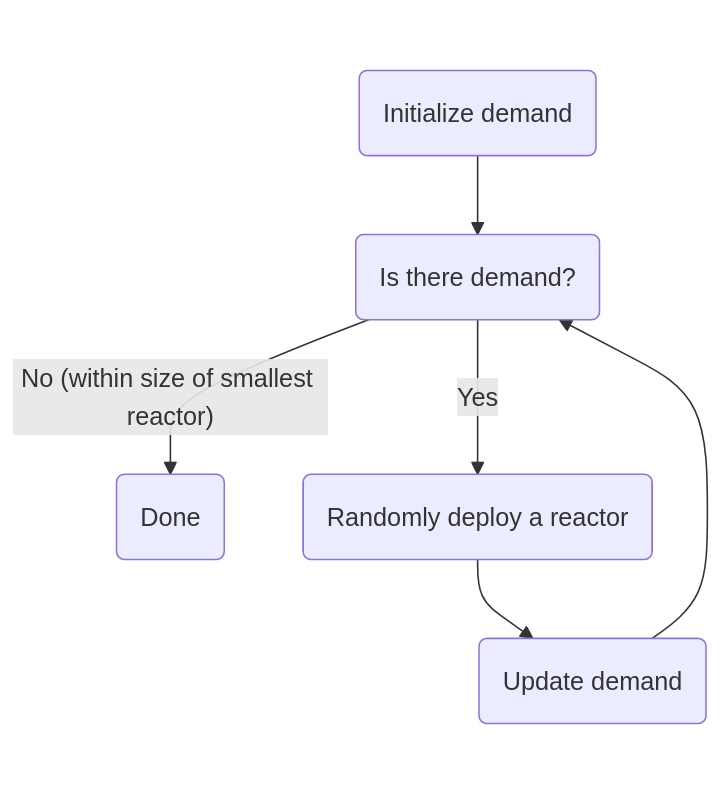
\includegraphics[scale=0.4]{images/schemes/random_diagram.png}
    \caption{Random Deployment Diagram}
    \label{fig:random_diagram}
\end{figure}

% when does it over or under perform


\section{Initially Random, Greedy Deployment}
% describe the algorithm in detail

\begin{figure}[!htbp]
    \centering
    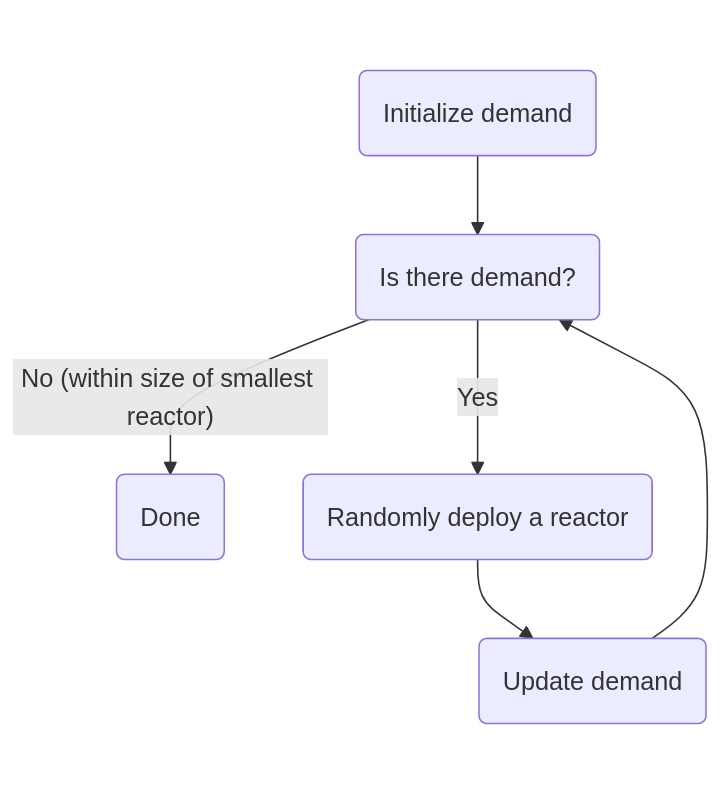
\includegraphics[scale=0.4]{images/schemes/random_diagram.png}
    \caption{Initially Random, Greedy Deployment Diagram}
    \label{fig:init_random_greedy_diagram}
\end{figure}

% what are the realistic and the unrealistic parts

% when does it over or under perform

